\chapter{ANÁLISES E RESULTADOS} % (fold)
\label{cha:analises_e_resultados}

\section{Introdução}
\label{cha:introducao}

 A análise dos resultados consistiu na elaboração de gráficos e tabelas com os dados retirados da base do experimento realizado. Os seguintes dados foram considerados para a análise:
 
\begin{itemize}
	\item Grupos de usuários
	
	\subitem Para se ter noção dos laços de amizades entre os participantes cadastrados no experimento. São 12 grupos no total, sendo que cada um deles possui no máximo 5 pessoas.
	
	\item Recomendações realizadas por amigos
	
	\subitem Informações dos produtos que foram recomendados na etapa 3 do experimento, onde os participantes deveriam recomendar 5 produtos a cada amigo presente no seu grupo. Cada participante possui no máximo 20 recomendações, sendo que alguns possuem apenas 15 devido à desistência de participantes do seu grupo.
	
	\item Recomendações realizadas por desconhecidos
	
	\subitem Informações dos produtos que foram recomendados na etapa 4 do experimento, onde os participantes deveriam recomendar 1 produto a alguns participantes de diferentes grupos, considerados desconhecidos. Cada participante possui no máximo 10 recomendações realizadas por desconhecidos, sendo que alguns possuem menos de 10 recomendações devido à desistência de participantes no experimento.
	
	\item Recomendações realizadas pelo sistema
	
	\subitem Todas as recomendações que o sistema realizou para os participantes. Contém a informação de qual participante recebeu a recomendação e qual foi o produto recomendado.
	
	\item Avaliação prevista do produto pelo sistema
	
	\subitem Ao recomendar um produto a um participante, o sistema calcula uma nota prevista para o mesmo. Essas informações foram armazenadas e consideradas durante a análise e exposição dos dados do experimento.
	
	\item Avaliações dos produtos
	
	\subitem Todas as avaliações de produtos no sistema. Contém os produtos avaliados na duas primeiras etapas do experimento, quando os participantes avaliaram 20 produtos em comum e 10 produtos de seu interesse, e as avaliações de produtos recomendados tanto pelos participantes como pelo sistema.
	
	\item Algoritmo utilizado para a recomendação
	
	\subitem Dentre as recomendações realizadas pelo sistema, foi retirada da base de dados a informação de qual algoritmo foi utilizado para gerar a recomendação.
	
\end{itemize}

 De posse dos dados, foram feitas as seguintes análises:
 
\begin{itemize}
	\item Análise Comparativa dos Algoritmos de Recomendação
	\item Análise de Rejeição das Recomendações
	\item Taxa de Serendipidade
	\item Análise do Algoritmo Baseado em Confiança
\end{itemize}

 Cada análise será discutida nas seções a seguir.
 
\section{Análise Comparativa dos Algoritmos de Recomendação}
\label{sec:analise_comparativa_dos_algoritmos_de_recomendacao}



\begin{figure}
    \centering
    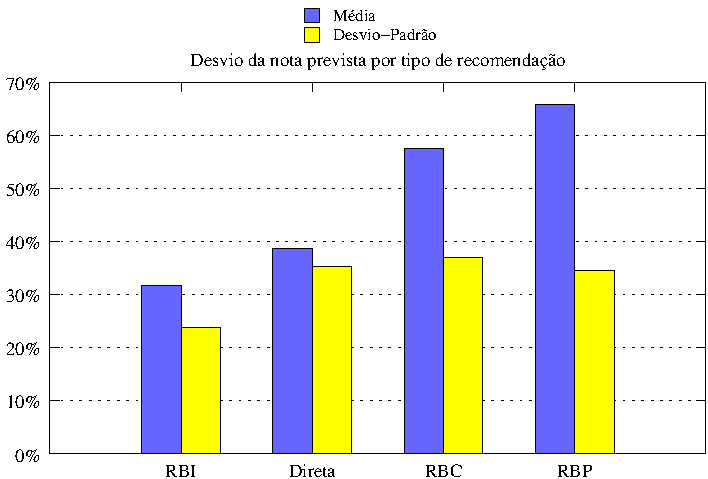
\includegraphics[width=\textwidth]{imagens/grafico_erro}
    \caption{\it Desvio da nota prevista por tipo de recomendação}
    \label{fig:erro}
\end{figure}

\begin{table}
\centering
\begin{tabular}{|r|c|c|}
    \hline
    Tipo de recomendação & Média& Desvio-Padrão \\
\hline 
Direta & 38.5952208545 & 35.2309513597 \\
\hline 
RBC & 57.3979591837 & 36.9792384652 \\
\hline 
RBI & 31.6068573222 & 23.7537026572 \\
\hline 
RBP & 65.8 & 34.5378053732 \\
\hline        
\end{tabular}
\caption{\it Desvio da nota prevista por tipo de recomendação}
\label{table:erro}
\end{table}


\begin{figure}
    \centering
    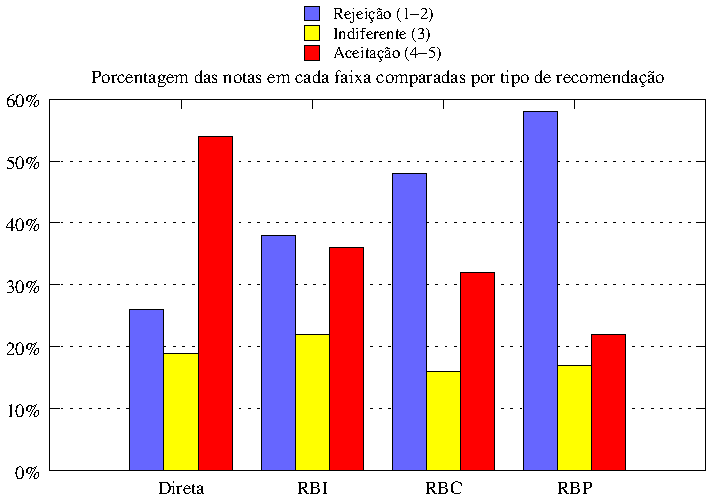
\includegraphics[width=\textwidth]{imagens/grafico_notas}
    \caption{\it Porcentagem das notas em cada faixa comparadas por tipo de recomendação}
    \label{fig:notas}
\end{figure}

\begin{table}
\centering
\begin{tabular}{|r|c|c|c|}
    \hline
    Tipo de recomendação & 1-2& 3& 4-5 \\
\hline 
Direta & 26 & 19 & 54 \\
\hline 
RBC & 48 & 16 & 32 \\
\hline 
RBI & 38 & 22 & 36 \\
\hline 
RBP & 58 & 17 & 22 \\
\hline        
\end{tabular}
\caption{\it Porcentagem das notas em cada faixa comparadas por tipo de recomendação}
\label{table:notas}
\end{table}


\begin{figure}
    \centering
    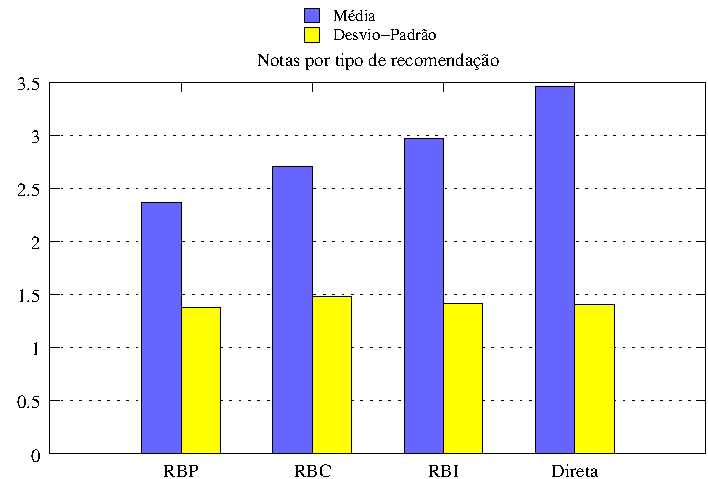
\includegraphics[width=\textwidth]{imagens/grafico_notas_medias}
    \caption{\it Notas por tipo de recomendação}
    \label{fig:notas_medias}
\end{figure}

\begin{table}
\centering
\begin{tabular}{|r|c|c|}
    \hline
    Tipo de recomendação & Média& Desvio-Padrão \\
\hline 
Direta & 3.45619116582 & 1.40923805439 \\
\hline 
RBC & 2.70408163265 & 1.47916953861 \\
\hline 
RBI & 2.964 & 1.41092310209 \\
\hline 
RBP & 2.368 & 1.38151221493 \\
\hline        
\end{tabular}
\caption{\it Notas por tipo de recomendação}
\label{table:notas_medias}
\end{table}


\begin{figure}
    \centering
    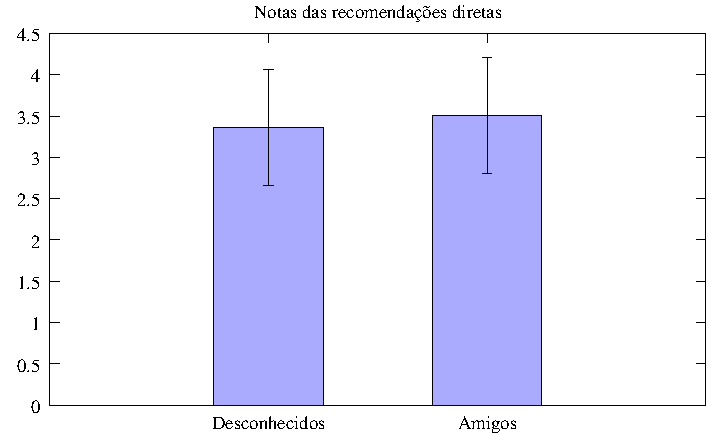
\includegraphics[width=\textwidth]{imagens/grafico_notas_medias_diretas}
    \caption{\it Notas das recomendações diretas}
    \label{fig:notas_medias_diretas}
\end{figure}

\begin{table}
\centering
\begin{tabular}{|r|c|c|}
    \hline
    Tipo de recomendação & Média& Desvio-Padrão \\
\hline 
Amigos & 3.50659340659 & 1.41167052454 \\
\hline 
Desconhecidos & 3.35881104034 & 1.39939396512 \\
\hline        
\end{tabular}
\caption{\it Notas das recomendações diretas}
\label{table:notas_medias_diretas}
\end{table}


\begin{figure}
    \centering
    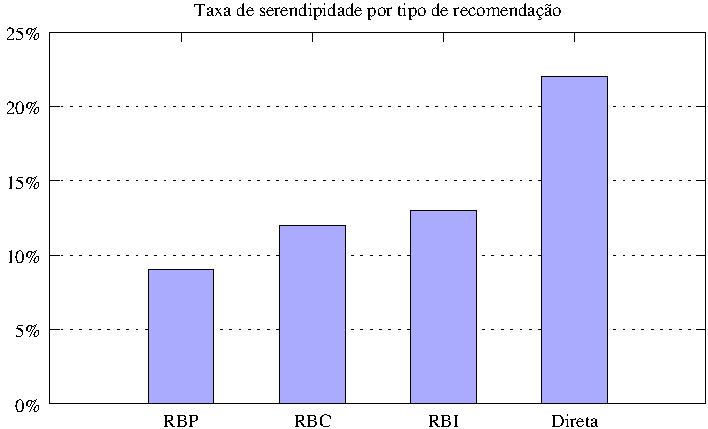
\includegraphics[width=\textwidth]{imagens/grafico_serendipidade}
    \caption{\it Taxa de serendipidade por tipo de recomendação}
    \label{fig:serendipidade}
\end{figure}

\begin{table}
\centering
\begin{tabular}{|r|c|}
    \hline
    Tipo de recomendação & Taxa de Serendipidade \\
\hline 
Direta & 22 \\
\hline 
RBC & 12 \\
\hline 
RBI & 13 \\
\hline 
RBP & 9 \\
\hline        
\end{tabular}
\caption{\it Taxa de serendipidade por tipo de recomendação}
\label{table:serendipidade}
\end{table}


\begin{figure}
    \centering
    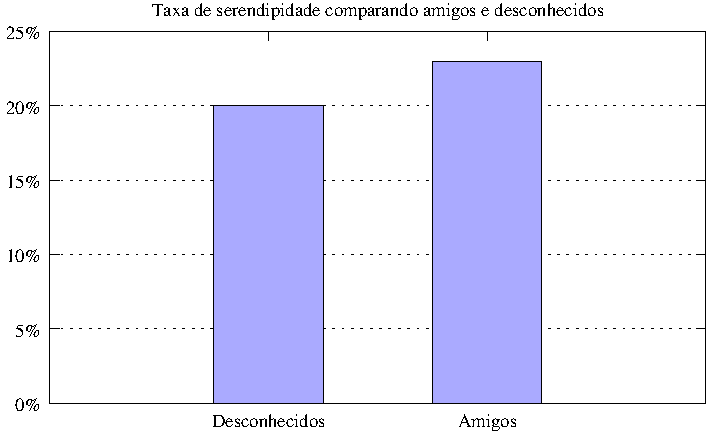
\includegraphics[width=\textwidth]{imagens/grafico_serendipidade_diretas}
    \caption{\it Taxa de serendipidade comparando amigos e desconhecidos}
    \label{fig:serendipidade_diretas}
\end{figure}

\begin{table}
\centering
\begin{tabular}{|r|c|}
    \hline
    Tipo de recomendação & Taxa de Serendipidade \\
\hline 
Amigos & 23 \\
\hline 
Desconhecidos & 20 \\
\hline        
\end{tabular}
\caption{\it Taxa de serendipidade comparando amigos e desconhecidos}
\label{table:serendipidade_diretas}
\end{table}


 
\subsection{Recomendações do Sistema}

\subsection{Recomendações Diretas}

% section analise_comparativa_dos_algoritmos_de_recomendacao (end)

\section{Análise de Rejeição das Recomendações}
\label{sec:analise_de_rejeicao_das_recomendacoes}

\subsection{Recomendações do Sistema}

\subsection{Recomendações Diretas}

% section analise_de_rejeicao_das_recomendacoes (end)

\section{Taxa de Serendipidade}
\label{sec:taxa_de_serendipidade}

% section taxa_de_serendipidade (end)

\section{Análise do Algoritmo Baseado em Confiança}
\label{sec:analise_do_algoritmo_baseado_em_confianca}

% section analise_do_algoritmo_baseado_em_confianca (end)

\section{Análise de Desempenho}
\label{sec:analise_de_desempenho}
% TODO falar sobre os problemas enfrentados com as consultas SQL e com as estrelinhas para a avaliação do produto (javascript).

Durante a realização do experimento algumas requisições ao servidor de aplicação foram identificadas como gargalo de desempenho do sistema. Ao analisar estas requisições, foi possível verificar que o fatores responsáveis pela degradação da performance estavam relaciondos ao tempo e quantidade das requsições ao banco de dados. As consultas SQL na tabela de produtos, com cerca de cento e vinte mil registros, foram as principais responsáveis pelo aumento no tempo de resposta. Esses problemas de performance foram rapidamente corrigidos através da redução do número de requisições ao banco de dados e pela paginação dos resultados. Os tempos de resposta das requisições antes da otmização das consultas podem ser observados na Tabela~\ref{table:before_stats} e comparados com os valores obtidos após a otmização na Tabela~\ref{table:after_stats}.

\begin{table}\centering
\begin{tabular}{|c|c|c|c|c|}
\hline
\textbf{Requisção Web}
& \textbf{Média}
& \textbf{Desvio Padrão}
& \textbf{Min.} 
& \textbf{Max.} \\ \hline
ProductsController\#index.html [GET]    & 16.90s & 29.02s &  0.00s &  5m06s \\
\hline
ProductsController\#rate.html [POST]    &  2.09s &  1.24s &  0.80s & 32.16s \\
\hline
ProductsController\#unknown.html [POST] &  1.26s &  0.54s &  0.85s &  2.42s \\
\hline
ProductsController\#show.html [GET]     &  1.18s &  1.21s &  0.00s &  8.52s \\
\hline
\end{tabular}
\caption{\it Tempo de resposta das requisições ao banco de dados antes da otimização \label{table:before_stats}}
\end{table}

\begin{table}\centering
\begin{tabular}{|c|c|c|c|c|}
\hline
\textbf{Requisção Web}
& \textbf{Média}
& \textbf{Desvio Padrão}
& \textbf{Min.} 
& \textbf{Max.} \\ \hline
ProductsController\#index.html [GET]    & 1.28s &  3.51s &  0.00s & 57.42s \\
\hline
ProductsController\#rate.html [POST]    & 0.13s &  0.77s &  0.00s & 21.05s \\
\hline
ProductsController\#unknown.html [POST] & 0.02s &  0.10s &  0.00s &  2.66s \\
\hline
ProductsController\#show.html [GET]     & 0.02s &  0.12s &  0.00s &  1.99s \\
\hline
\end{tabular}
\caption{\it Tempo de resposta das requisições ao banco de dados após a otimização \label{table:after_stats}}
\end{table}

Para completar a análise da performance do sistema, a Tabela~\ref{table:process_blockers} apresenta as requisições bloqueantes, isto é, aquelas com duração total maior do que um segundo. Os dados apresentados na Tabela~\ref{table:process_blockers} são referentes apenas as requisições feitas após a otimização até o término do experimento.

\begin{table}\centering
\begin{tabular}{|c|c|c|}
\hline
\textbf{Requisção Web}
& \textbf{Ocorrências}
& \textbf{Porcentagem} \\ \hline
UserRecommendationsController\#new.html [GET]     & 1596 & 65.2\% \\ 
\hline
ProductsController\#index.html [GET]              &  315 & 12.9\% \\ 
\hline
AdminController\#index.html [GET]                 &  167 &  6.8\% \\
\hline
ProductsController\#rate.html [POST]              &  165 &  6.7\% \\
\hline
HomeController\#index.html [GET]                  &  128 &  5.2\% \\ 
\hline
UserRecommendationsController\#create.html [POST] &   38 &  1.6\% \\
\hline
RecommendationGuidesController\#index.html [GET]  &   11 &  0.4\% \\  
\hline
InvitationsController\#create.html [POST]         &    8 &  0.3\% \\  
\hline
ProductsController\#unknown.html [POST]           &    8 &  0.3\% \\  
\hline
RatingsController\#index.html [GET]               &    7 &  0.3\% \\  
\hline
SessionsController\#create.html [POST]            &    4 &  0.2\% \\  
\hline
UsersController\#new.html [GET]                   &    1 &  0.0\% \\  
\hline
ProductsController\#show.html [GET]               &    1 &  0.0\% \\
\hline
\end{tabular}
\caption{\it Requisições bloqueantes \label{table:process_blockers}}
\end{table}


% section analise_de_desempenho (end)
